\documentclass[a4paper,12pt]{article}
\usepackage{fancyhdr}
\usepackage{graphicx}
\usepackage[utf8]{inputenc}


\title{Project Plan}
\author{Group Project 3 - Group 2}
\date{March 4 2008}

\begin{document}
\maketitle
\newpage
\tableofcontents
\newpage

\section{Introduction}
After definining the scope of our project, planning the work is a necessary step to drive the project forward and achieve the objectives.
We must also share the work in an efficient and fair way between our members, and find a way to work together and share the different resources.

\section{Main steps and workload}
\subsection{Setting up}
Because our project will be written with the Groovy/Rails language and development framework, which is totally new for us,
we need some time to set up a development environment and ready ourselves to use this new technology.
\subsection{Design}
Designing our application will probably be the main task of the project.
Despite already having the beginnings of a specification before we started our project, it will be an important and critical task.
\subsection{Coding}
The coding is usually 30\% of the total project effort. In our case we can't define a precise workload for this task. Most of the coding effort will be due to the user interface.
So the level to which we refine the user interface will depend on the time we have left.

But in order to build the core of our project with a basic user interface, we predict that the coding will not be more than 20\% of our total project effort.
\subsection{Testing}
The testing of our software will be done during the development. We are not going to test the software only when it is finished, but during the whole development process, with unit testing.
We plan only a short final user test at the end of the project.
\subsection{Documentation writing}
50\% of our mark will be the result of our documentation, and this documentation is also a good communication tool between team members.
We really think that documentation writing is an important part of our project and we will include it during the whole project process.
\newpage
\subsection{Gantt Chart}
\begin{center}
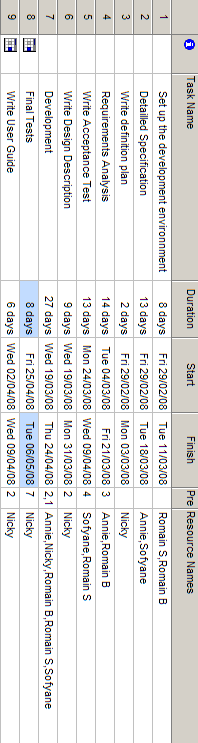
\includegraphics[scale=0.7]{ressources.png}
\end{center}
\newpage
\begin{center}
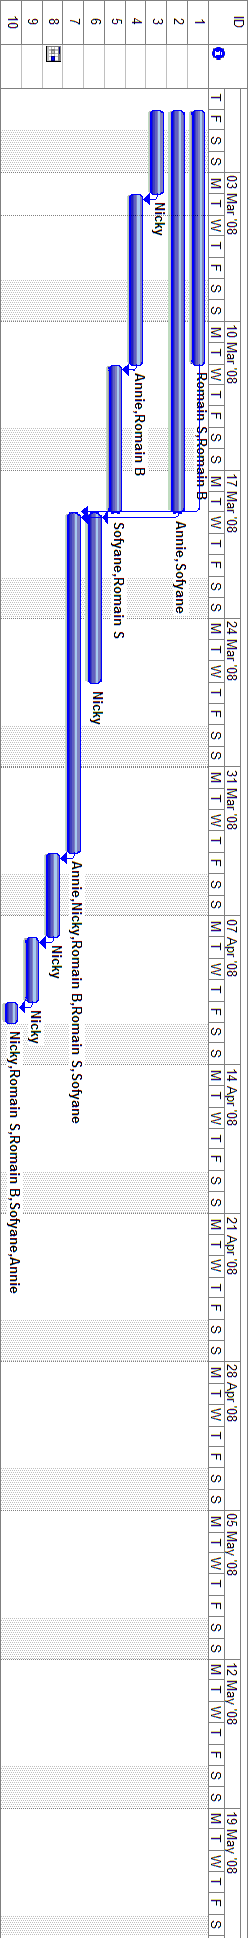
\includegraphics[scale=0.40]{gantt.png}
\end{center}
\newpage
\section{Collaborative work}
Working efficiently in a team with shared resources is always a problem, that is why we have to use all the tools which are available to us, and ensure good communication between members of the group.

We have a weekly half hour group meeting with our supervisor. The main aim of this meeting is to inform our supervisor of our work and to benefit from his advices.
Additionally we have a 3 hour group meeting every Friday, this gives the members an opportunity to communicate, find out the problems in the project and solve them.

One issue in collaborative development is working on the same documents at the same time. To help us do this, we are going to use a source version control system, called SVN, which is available for free on the Google Code's platform. This system will allow us to work together on the same files simultaneously, and keep a log of all the changes. It will also be a place where all of our work will be backed up.
As for the documentation, we are already using Google Docs, which provides us with a friendly collaborative document editing system.

\section{Development method}
Because the scope of our project is maybe too much for the time we have, we have chosen to use an iterative and prototype based development method.
This kind of method allows us to have a fully functional version of our project at the end of each iteration. And we refine the software after each iteration.
It's mainly a way for us to reduce the risk of not being able to hand in a functional project because of the time constraint.

Moreover, the Grails Framework has various prototyping features that will help us a lot in using this approach.

\section{Team management}
Our team members have all very different skills and technological background. So we have tried to share the work according to abilities of each.
\begin{itemize}
\item Romain Bossut: Project Leader, specialized in project management and coding.
\item Abou Sofyane Khedim: Team worker, specialized in design and coding.
\item Romain Sacchettini: Team worker, specialized in coding.
\item Nicholas Ward: Team worker, specialized in coding and documentation writing.
\item Annie Lai Cheung: Team worker, specialized in design and coding.
\end{itemize}

Despite the specialization of each member, we want to give an opportunity to each member to have a look at the Groovy and Rails technology and learn something new,
so the whole team is going to work on the coding process.

\section{Conclusion}
Because of the time constraint, we have to stick to this plan to be able to complete the module. Moreover this project plan is a kind of contract between each member of the group and it sets up the duties of each member.
However, a plan is never a religion and it might be revised at any moment with the agreement of the whole group.

\end{document}

